% Kapitel 1 -- Einleitung (Stand: Version 2.0.0)
\section{Einleitung}\label{sec:einleitung}
AES wurde von Joan Daemen und Vincent Rijmen (unter dem Alias Rijndael) entwickelt und ist als Advanced Encryption Standard in \cite{fips197} festgeschrieben. Es basiert auf dem Prinzip der symmetrischen Verschlüsselung, bei der derselbe Schlüssel zum Ver- und zum Entschlüsseln dient, und gilt mit seinen verschiedenen Standards als eines der besten Verschlüsselungsverfahren der Welt. Dies ist bedingt durch die Tatsache, dass bis heute kein effektiver Algorithmus gefunden wurde, welcher die Brute-Force-Methode zum Entschlüsseln des Chiffretextes umgeht. Da in absehbarer Zeit die Prozessorleistung keinen sonderlichen Leistungsschub mehr erhalten wird, ist die Schlüssellänge für die Sicherheit ausschlaggebend; also die Dauer der Entschlüsselung.

\subsection{Was dieses Programm umsetzt}
Die hier als Assemblerprogramm (TASM, Prozessor \asm{.486}, Ausführung in der DOS-Box) umgesetzte Variante beruht auf dem Grundgedanken von AES, \emph{ist aber nicht AES nach \cite{fips197}}. Sie arbeitet nicht mit einem einzelnen 16-Byte-Block, sondern mit einem \emph{Zustand} aus 64 Bytes, der in vier unabhängige $4\times4$-Blöcke gegliedert ist (Abschnitt~\ref{sec:zustand}). Der Schlüssel hat ebenfalls 64 Bytes à 8~Bit (also je Stelle 256 mögliche Werte, $0\ldots255$, was der erweiterten ASCII-Tabelle entspricht). Tabelle~\ref{tab:vergleich} stellt den Standard der umgesetzten Variante gegenüber.

\begin{table}[!htbp]
    \centering
    \small
    \renewcommand{\arraystretch}{1.15}
    \caption{AES nach FIPS-197 im Vergleich zur Umsetzung in Version \versionProjekt}\label{tab:vergleich}
    \begin{tabular}{@{}p{3.2cm}p{4.9cm}p{5.4cm}@{}}
        \toprule
        & \textbf{AES (FIPS-197)} & \textbf{diese Umsetzung} \\
        \midrule
        Blockgröße & 16 Byte (ein $4\times4$-Block) & 64 Byte, als vier unabhängige $4\times4$-Blöcke \\
        Schlüssellänge & 128, 192 oder 256 Bit & 64 Byte (512 Bit); Standardschlüssel eingebaut, eigener Schlüssel eingebbar \\
        Rundenzahl & 10, 12 oder 14 & 2 Runden mit abschließender S-Box-Stufe (aktiver Ablauf) \\
        SubBytes & S-Box & identisch (AES-S-Box, 256 Einträge) \\
        ShiftRows & Zeile $r$ um $r$ Stellen nach links & identisch, je Block \\
        MixColumns & in jeder Runde außer der letzten & als \asm{ShiftColumn} und \asm{ShiftColumn_1} vorhanden, im aktiven Ablauf \emph{nicht} aufgerufen \\
        Schlüsselexpansion & wortweise, \asm{RotWord}/\asm{SubWord}, \asm{Rcon} & eigenes Verfahren: Byte-Präfix-XOR mit S-Box-Wert und rotierender Konstante (\asm{5Fh}) \\
        \bottomrule
    \end{tabular}
\end{table}

Daraus folgt: Das Verfahren ist \emph{AES-ähnlich} und \textbf{nicht für den Schutz echter Daten geeignet}. Ohne MixColumns im aktiven Ablauf gibt es keine Diffusion; ein Klartextbyte beeinflusst genau ein Chiffrebyte (Kapitel~\ref{sec:einschraenkungen}). Der Zweck des Projekts ist, die Bausteine von AES in Assembler nachzuvollziehen und im Detail zu verstehen.

Die folgenden Schemata zeigen den \emph{AES-Standardablauf} als Vorbild. Welche Schritte das Programm tatsächlich in welcher Reihenfolge ausführt, steht in Kapitel~\ref{sec:ablauf-beispiel} und in den Abschnitt~\ref{sec:ablauf-v} und~\ref{sec:ablauf-e}.

\begin{figure}[!htbp]
    \centering
    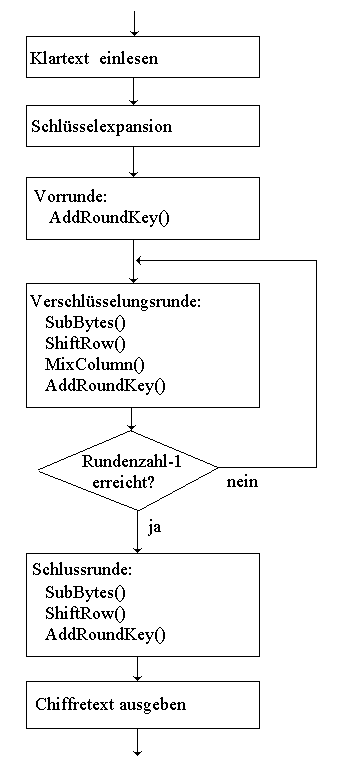
\includegraphics[height=0.5\textheight,keepaspectratio]{images/schema_verschluesselung.png}
    \caption{Schema Verschlüsselung mit AES (Standardablauf) -- Quelle: \cite{ceilers_ver}}
    \label{fig:schema-ver-1}
\end{figure}

\begin{figure}[!htbp]
    \centering
    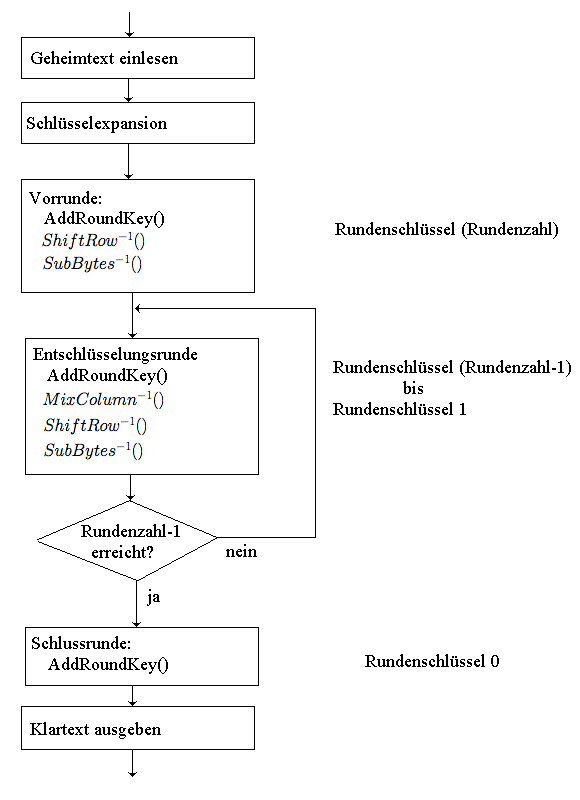
\includegraphics[height=0.5\textheight,keepaspectratio]{images/schema_entschluesselung.png}
    % Im PDF stand hier faelschlich ebenfalls "Verschluesselung".
    \caption{Schema Entschlüsselung mit AES (Standardablauf) -- Quelle: \cite{ceilers_ent}}
    \label{fig:schema-ent-1}
\end{figure}

\subsection{Versionen}
Dieses Dokument beschreibt die \textbf{Version \versionProjekt} (Branch \texttt{v2.0.0}). Die ursprüngliche Abgabe aus dem Jahr 2021 ist die \emph{Version 1.0} (Stand im Git: Commit \commit{89f8212}). Sie wurde damals in fünf getrennten PDF-Dokumenten beschrieben; diese Beschreibungen sind in dieses Dokument eingearbeitet und auf den Stand~\versionProjekt\ gebracht worden. Was sich gegenüber Version~1.0 geändert hat, steht gesammelt in Kapitel~\ref{sec:aenderungen}; die zugehörige Erklärung der Autoren in Kapitel~\ref{sec:erklaerung}.

\subsection{Aufbau dieses Dokuments}
\begin{description}[leftmargin=!,labelwidth=3.4cm,noitemsep]
    \item[Kapitel~\ref{sec:grundlagen}] Datenmodell, Rechnen in $\mathrm{GF}(2^8)$, Registerrollen und Bildschirmadressen -- die Grundlagen, die alle weiteren Kapitel voraussetzen.
    \item[Kapitel~\ref{sec:asm-dateien}] Jede ASM-Datei, jede \asm{PROC} und jedes wichtige Label, mit Registern und Befehlen.
    \item[Kapitel~\ref{sec:ablauf-beispiel}] Ein durchgehendes Zahlenbeispiel (Klartext \glqq Hallo\grqq) durch alle Schritte.
    \item[Kapitel~\ref{sec:batch}--\ref{sec:einschraenkungen}] Batch-Dateien, Bedienung, Funktionsumfang und bekannte Einschränkungen.
    \item[Kapitel~\ref{sec:aenderungen}--\ref{sec:tests}] Änderungen in Version~\versionProjekt, Entwurfsskizze und Tests.
    \item[Kapitel~\ref{sec:erklaerung}] Erklärung der Autoren.
\end{description}
